\newpage
\section{Create two functions in R and compute the GMM with the S\&P500 returns}

Adopting the exact same approach as previous, moment conditions are defined as follows:
\begin{equation*}
    Y=    
    \begin{bmatrix}[l]
    E[X^2]-\frac{\nu}{\nu-2} \\
    E[X^4]-E[X^2]^2(\frac{6}{\nu-4}+3)
    \end{bmatrix}
\end{equation*}

The function returns the scalar resulting from the quadratic form $Y^TWY$. However, in this particular case, the S\&P500 sample of returns is used. The methodology is the same as before: minimizing the moment conditions with respect to $\nu$. The following quadratic form is solved for different parameter candidates and two weight matrices ($W_1=I$ and $W_2=\Sigma^{-1}$).
\begin{equation*}
    Y^TWY
\end{equation*}
\begin{equation*}
    W_1=
    \begin{bmatrix}
        1   &0 \\
        0   &1
    \end{bmatrix};\;\;\;\;\;
    W_2=\Sigma^{-1}=
    \begin{bmatrix}[l]
        \frac{1}{\sigma_{m_1,m_1}}    &\frac{1}{\sigma_{m_1,m_2}} \\
        \frac{1}{\sigma_{m_2,m_1}}    &\frac{1}{\sigma_{m_2,m_2}}
    \end{bmatrix}
\end{equation*}

Running the code for the two cases generate a vector containing the output of the minimization problem for every parameter $\nu$ employed. Recall that by the first moment condition $\nu>4$ therefore a parameter list of the following form is set: $\nu_i \in \{5:30\}$. The goal is to find the parameter $\nu$ for which the objective function, i.e. criterion, is minimized, Figures 1.5 and 1.6 illustrate the result.
\bigskip\par
The data used in the exercise gives an estimated $\nu$ of:
\begin{equation*}
    \begin{cases}
    \widehat{\nu}_{GMM_{1}}=5 \;\;\text{using W=I}\\
    \widehat{\nu}_{GMM_{2}}=30 \;\;\text{using W=}\Sigma^{-1}
\end{cases}
\end{equation*}


Estimates differ depending on the weight matrix involved in the optimization problem. The first case might be a "naive" estimate given that equal weight is attributed to the moment conditions.  When using the inverse of the covariance matrix, we put more reasonable weights on the moments. The following sections discuss the difference between the two estimates.


\subsection{$W=I$}\label{SectionCriterionSP500_I}
The convexity of the objective function seems to have disappeared. The function has a minimum at $\nu_1=5$ and trying to run the code changing the candidates list to $\nu_i \in \{6:30\}$ won't change the result: the minimum will always be the first candidate tested. Chapter \ref{ChapterSP_I} aims to provide an explanation to this result.

\subsection{$W=\Sigma^{-1}$}\label{SectionCriterionSP500_W}
At first sight it seems correct to have convexity, the problem here is that the minimum is reached when running the optimization using the exact last candidate. Expanding the list of candidates from $\nu_i \in \{5:30\}$ to $\nu_i \in \{5:1000\}$ won't change the outcome, in this case the minimum would be at $\nu=1000$. To understand this result, the covariance matrix has to be analysed.
\begin{equation*}
    W=\Sigma=
    \begin{bmatrix}[r]
        31.84035    &8250.907 \\
        8250.90722  &2839215.102
        \end{bmatrix}
\end{equation*}
Notice that the variance associated to the second moment condition is 89170.3483 times bigger than the variance associated to the second moment condition. The problem arises when we calculate the objective function, in order to compute the output we have to invert $\Sigma$, therefore $\Sigma^{-1}$ is:
\begin{equation*}
    W^{-1}=\Sigma^{-1}=
    \begin{bmatrix}[r]
        \frac{1}{31.84035}    &\frac{1}{8250.907} \\
        \frac{1}{8250.90722}  &\frac{1}{2839215.102}
        \end{bmatrix}=
    \begin{bmatrix}[l]
        0.1271814035    &-3.695958\mathrm{e}{-04} \\
        -0.0003695958    &1.426275\mathrm{e}{-06}
    \end{bmatrix}
\end{equation*}
By using this approach the output almost fully depends on the second moment, the weight associated to the fourth moment is in fact almost negligible. The second moment condition (fourth moment) barely influences the optimization problem whilst solving the quadratic form and, as a result, the objective function is somewhat restricted to minimising the first moment condition (Second moment). In this particular case, minimising this condition seems to point towards the Normal Distribution being the best fit for the S\&P500 returns: the objective function asymptotically tends to 0 as the parameter increases.

\subsection{Estimated vs. theoretical density functions}
Figure 1.7 compares the estimated density function based on the S\&P500 data using $I$ as the weighting matrix with the theoretical Student t-distribution with 5 degrees of freedom, since $df=5$ gave the minimum value of the objective function.
\smallskip\par
Figure 1.8 compares the estimated density function based on the S\&P500 data using the covariance matrix between the two moment conditions as the weighting matrix with the theoretical Student t-distribution with 30 degrees of freedom, which again gives us the minimum value of the objective function. In both cases our estimate seems to be unbiased, centered around 0, but from the real data-set (black line) we get a taller and skinnier distribution than the theoretical distribution (red line).
\smallskip\par 
We could use a Goodness Of Fit Test to determine the validity of our assumption that returns follow a Student distribution, for example a $\chi^2$, Kolmogorov-Smirnov, or Anderson-Darling test to see whether there is significant difference between the two densities.




\begin{figure}
    \centering
    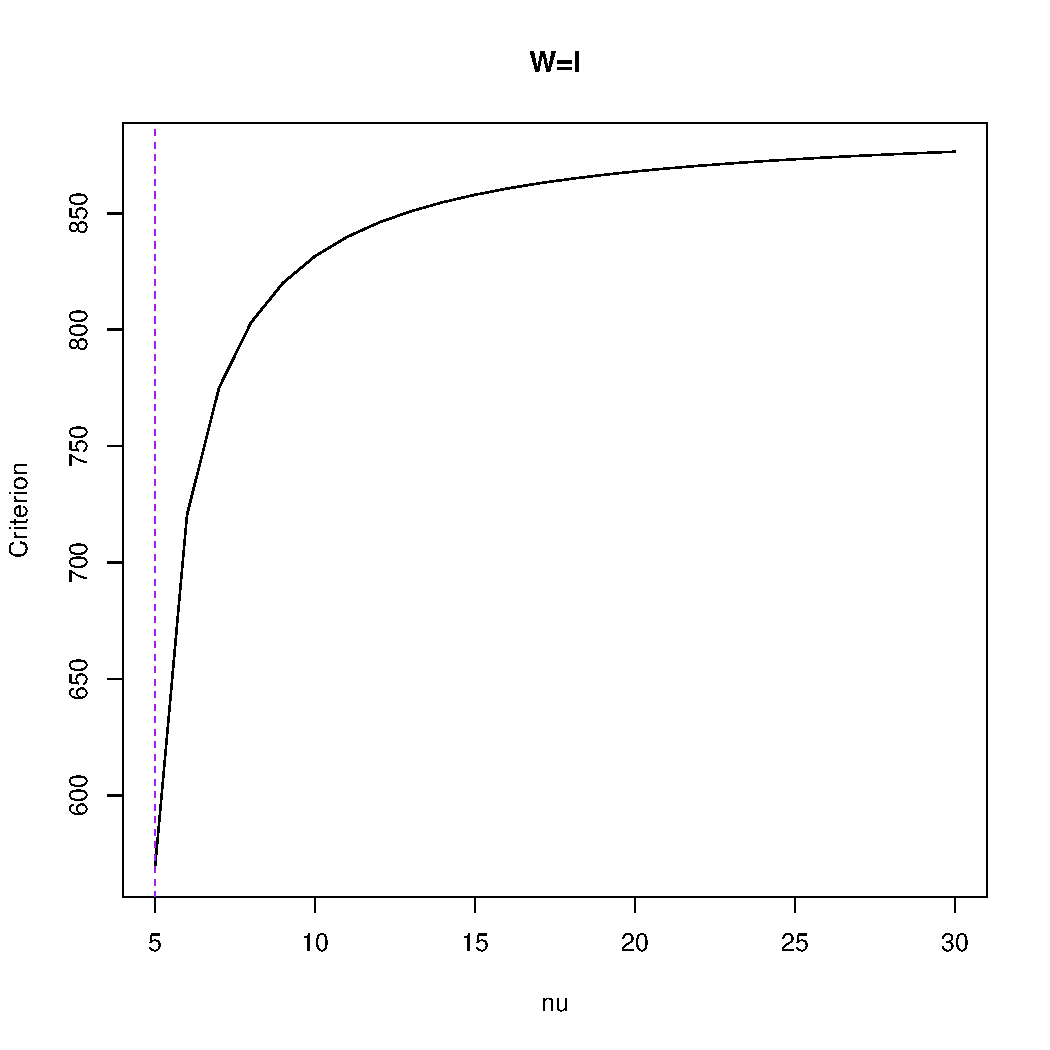
\includegraphics[width=0.7\textwidth]{S&P500_returns_criterion_(W=I).pdf}
    \label{SP500_returns_criterion_I}
    \caption{Output distribution as a function of the candidates $\nu$ using $W=I$}
    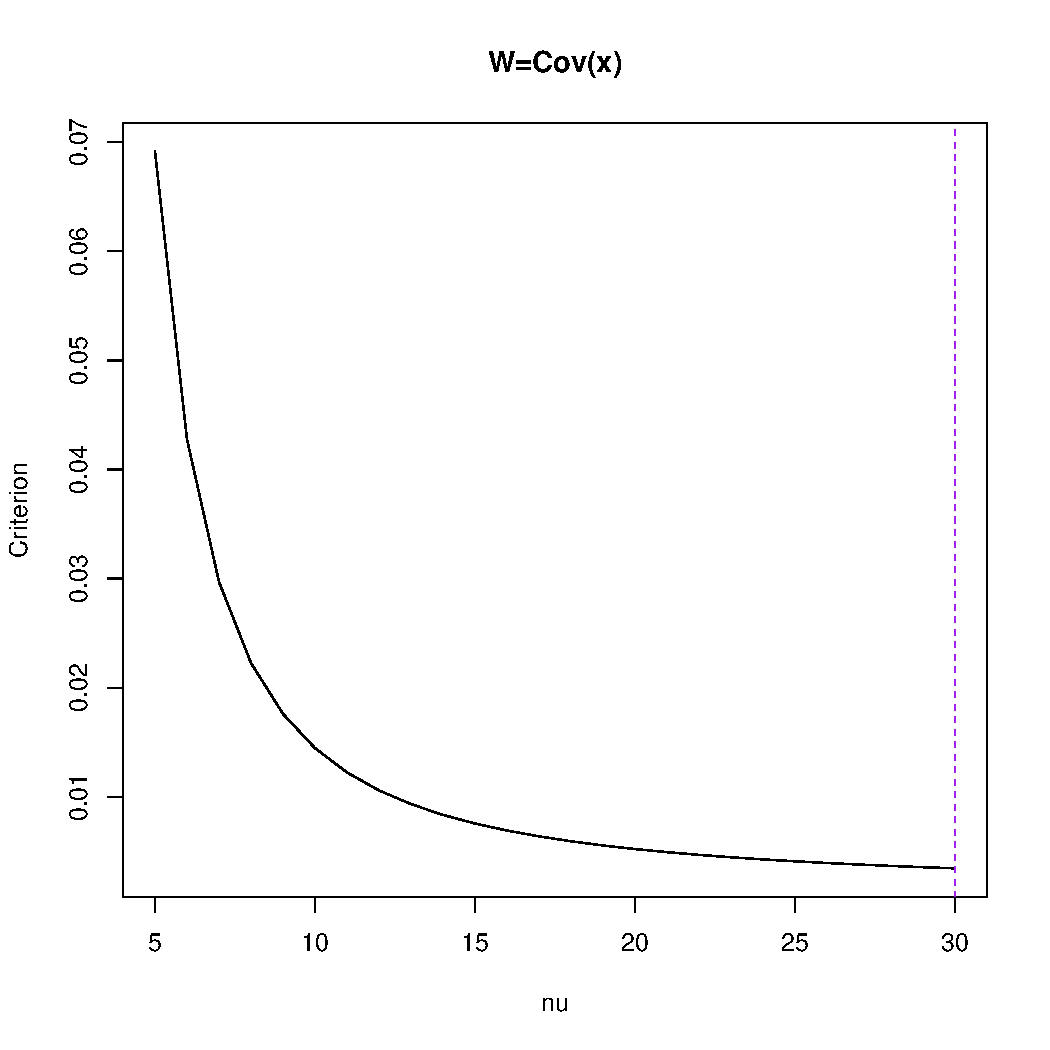
\includegraphics[width=0.7\textwidth]{S&P500_returns_criterion_(W=Sigma^-1).pdf}
    \label{SP500_returns_criterion_W}
    \caption{Output distribution as a function of the candidates $\nu$ using $W=\Sigma^{-1}$}
\end{figure}

\begin{figure}
    \centering
    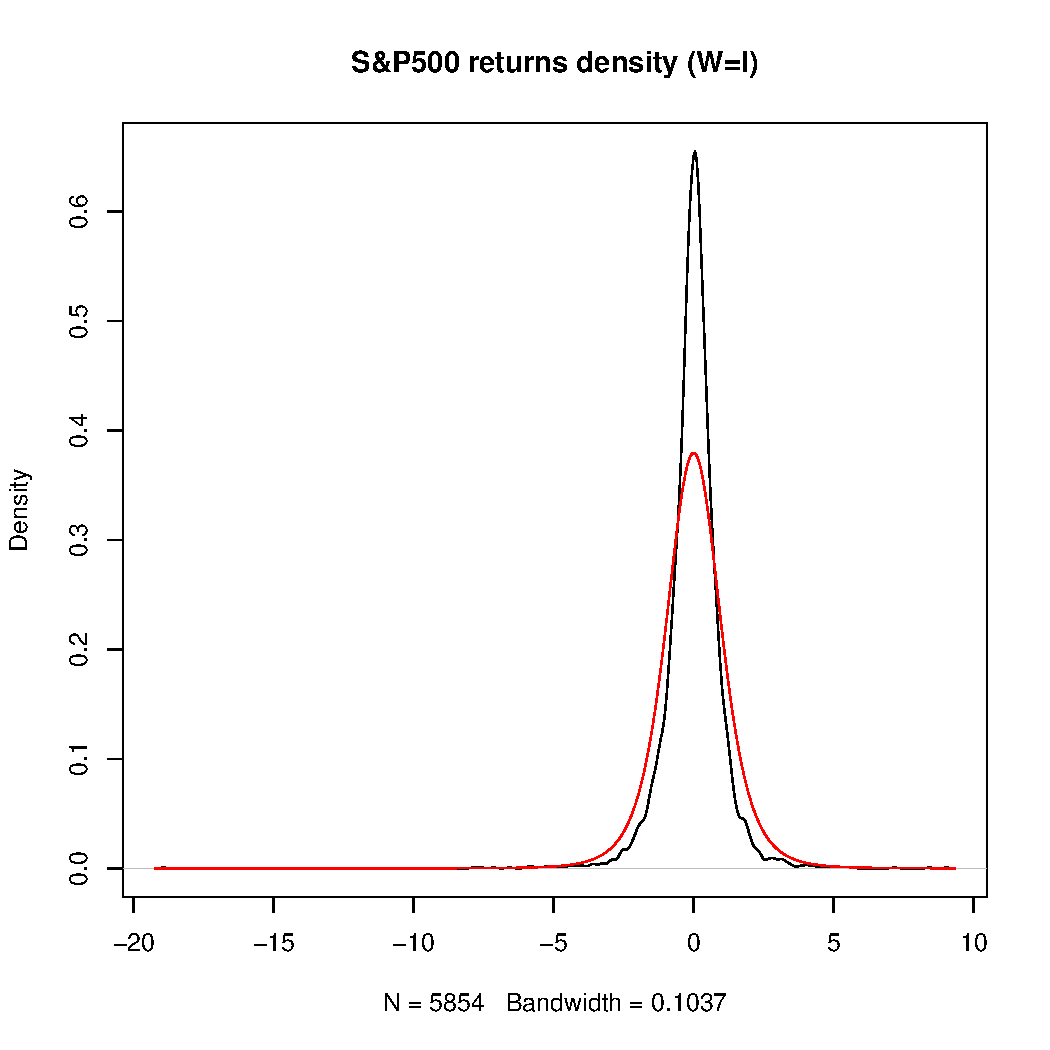
\includegraphics[width=0.7\textwidth]{S&P500_returns_density_(W=I).pdf}
    \label{SP500_returns_density_I}
    \caption{S\&P500 returns density using $W=I$}
    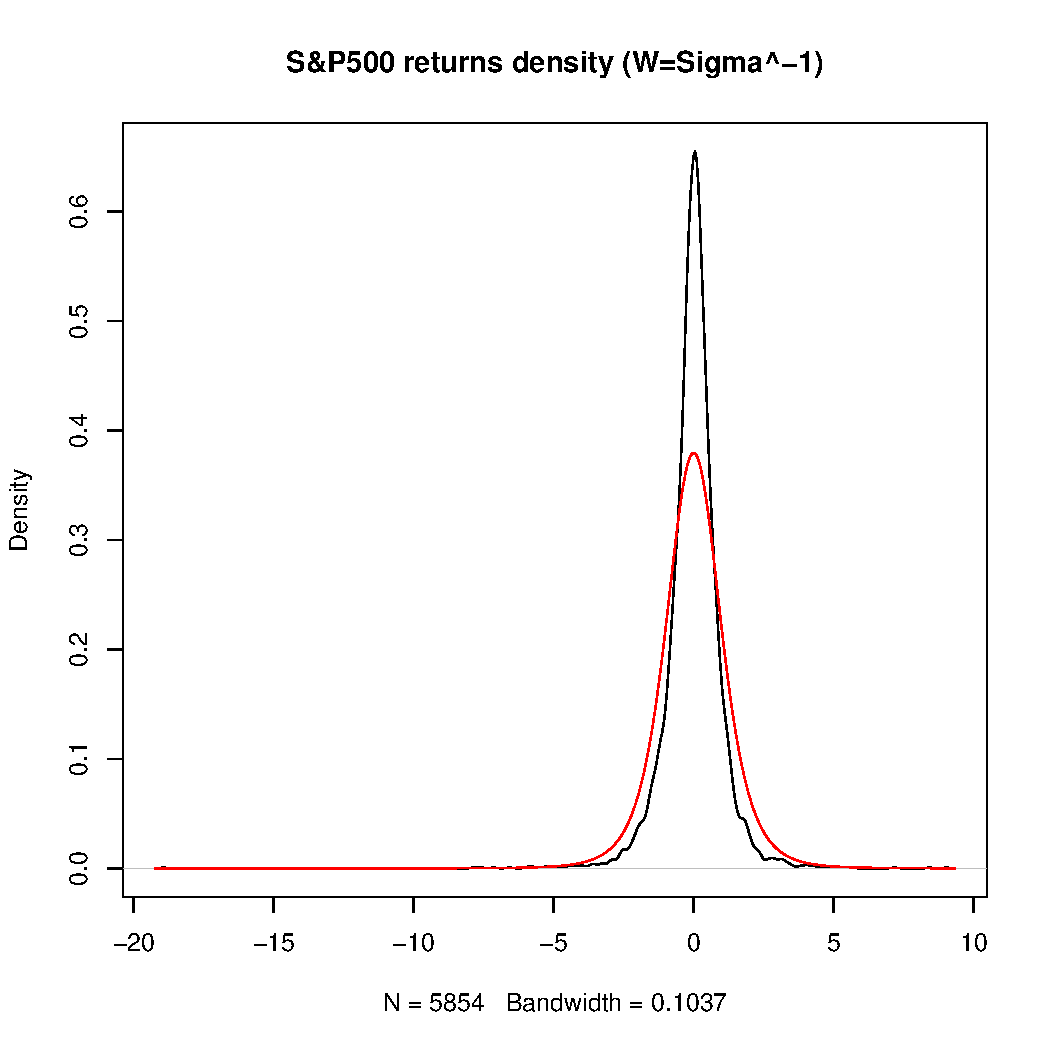
\includegraphics[width=0.7\textwidth]{S&P500_returns_density_(W=Sigma^-1).pdf}
    \label{SP500_returns_density_W}
    \caption{S\&P500 returns density using $W=\Sigma^{-1}$}
\end{figure}
